\documentclass[11pt,a4paper]{article}
\usepackage[utf8]{inputenc}
\usepackage[catalan]{babel}
\usepackage{amsmath}
\usepackage{amsfonts}
\usepackage{enumerate}
\usepackage{enumitem}
\usepackage{amssymb}
\usepackage{graphicx}
\usepackage{fancyhdr}
\usepackage{appendix}
\usepackage[hidelinks]{hyperref}
\usepackage{hyperref}
\usepackage{subfig}
\usepackage{float}
\usepackage[ampersand]{easylist}
\usepackage{multirow}
\usepackage{amsmath}
\usepackage{amsfonts}
\newcommand\tab[1][1cm]{\hspace*{#1}}
\usepackage[left=2cm,right=2cm,top=2cm,bottom=2cm]{geometry} 
\renewcommand{\appendixname}{Webgrafia}
\renewcommand{\appendixtocname}{Webgrafia}
\renewcommand{\appendixpagename}{Webgrafia}


\begin{document}
\begin{titlepage}

\begin{flushleft}
Escola Politècnica Superior\\
\vspace*{0.15in}
Grau en Enginyeria Informàtica\\
\vspace*{0.15in}
Automatic Reasoning and Learning
\end{flushleft}

\begin{center}
\vspace{2.0cm}

\includegraphics[scale=0.3]{Figures/M-UdL.jpg} 
\vspace{2.0cm}

\begin{LARGE}
\textbf{Pràctica de Models Probabilístics:}\\ 
\vspace*{0.15in}
Indentificació de classes de vidres en l'escena del crim
\end{LARGE}
\vspace{1.0cm}

\begin{large}
\textbf{Data}: 25 de Juny, de 2018 \\
\textbf{Professor}: Ramón Béjar Torres \\
\begin{tabular}{ll}
\textbf{Nom: }Marc Melis Batalla & \textbf{DNI: }48257130W \\
\textbf{Nom: }Roger Truchero Visa  & \textbf{DNI: }48056539V \\
\end{tabular}
\end{large}

\vspace*{0.2in}
\begin{center}
\rule{120mm}{0.1mm}\\
\end{center}
\end{center}
\vspace*{0.2in}
\part*{Objectius}
L'objectiu del treball és realitzar aprenentatge basat en xarxes bayesianes, en lloc de basat en sistemes
de regles. Es tracta del problema de classificació de diferents classes de vidres en funció de diferents
propietats físiques dels mateixos. Aquest és el valor que té cada un dels 11 atributs que trobareu
per cada instància (propietats d'un cristall correctament identificat) en el fitxer glass.data que es troba juntament amb la pràctica.
\end{titlepage}

\lhead[\thepage]{
\includegraphics[scale=0.05]{Figures/M-UdL.jpg}  }
\chead[]{\textbf{Pràctica de Models Probabilístics}}
\rhead[]{ARA}
\renewcommand{\headrulewidth}{0.5pt}
\renewcommand{\footrulewidth}{0.5pt}
\fancypagestyle{plain}{
\fancyhead[L]{}
\fancyhead[C]{}
\fancyhead[R]{\thepage}
\fancyfoot[L]{}
\fancyfoot[C]{}
\fancyfoot[R]{}
\renewcommand{\headrulewidth}{0pt}
\renewcommand{\footrulewidth}{0pt}
}
\pagestyle{fancy}
\vspace*{0.05in}

\tableofcontents

\newpage

\listoffigures
\vspace*{0.2in}
\listoftables

\newpage

\part{Parseig de dades}
Donat el problema ens hem trobat amb una sèrie de dades amb valors reals, però per tal de poder-los implementar dins d'una xarxa bayesiana necessitem discretitzar-los.\\\\ Per a fer-ho hem decidit utilitzar la llibreria \textit{pandas}\footnote{\url{https://pandas.pydata.org}} de \textit{python}. També hem afegit una primera línia al fitxer de les dades \texttt{glass.data.txt} amb l'identificador de columna donat per \texttt{glass.names.txt} per facilitar la lectura del document a \textit{pandas} i no haver-ho d'afegir a posteriori i eliminem la columna d'identificadors perquè no ens aporta informació útil i \textit{pandas} ja inclou els seus propis índexs.\\\\

\begin{figure}[H]
\centering
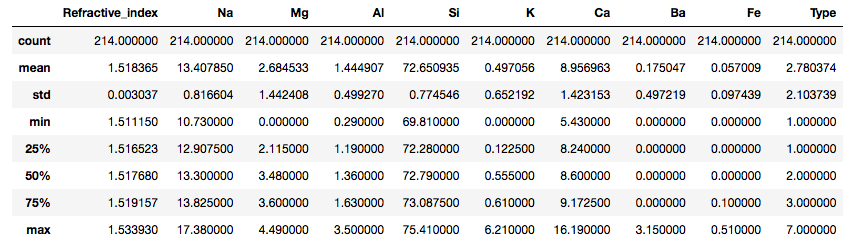
\includegraphics[width=\textwidth]{Figures/p1.png}
\caption{Tendència central, dispersió i forma de la distribució del conjunt de dades}
\end{figure}
\vspace*{0.2in}
Per tal de discretitzar els valors hem utilitzat la funció \texttt{pandas.cut}, que retorna els valors en diferents intervals segons el número de particions que imposis per paràmetre. Un cop tenim els intervals obtenim un diccionari amb, per cada interval, el número natural que li correspon de 0 fins al número d'intervals $-$ 1.\\

Un cop tenim els valors discretitzats afegim els camps necesaris pel format \texttt{.arff}. Afegim la relació i els atributs amb els seus rangs (tenin em compte que el camp \texttt{Type} no el discretitzarem ja que es un valor ja discret que va de 0 a 7. Finalment afegim les dades en format \texttt{csv} just a continuació i ja tenim el fitxer discretitzat i enllestit per passar-ho a \textit{Weka}.\\

L'script que em utilitzat es trobat al fitxer \texttt{src/data\_parsing.ipynb} com a una llibreta de \textit{Jupyter Notebook}\footnote{\url{http://jupyter.org}}.

\newpage

\part{Aprenentatge de models amb K2}
Abans de començar a apendre els models, haurem de carregar el fitxer \textit{.arff} que conté les dades dels materials del crim.\\
\begin{figure}[hbtp]
\centering
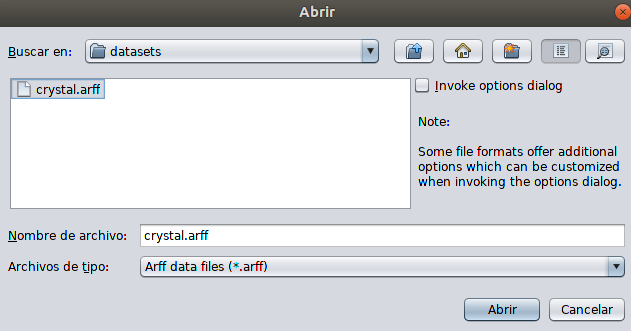
\includegraphics[scale=0.4]{Figures/1.png}
\caption{Selecció del fitxer de dades }
\end{figure}
\\\\
Seguidament seleccionar el classificador BayesNet:\\
\begin{figure}[hbtp]
\centering
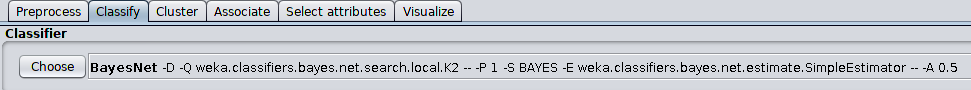
\includegraphics[scale=0.5]{Figures/2.png}
\caption{Classificador BayesNet}
\end{figure}
\\\\
I finalment, seleccionar l'algorisme d'aprenentatge K2 per, posteriorment, modificar-ne els seus paràmetres d'execució i poder obtenir diferents tipus de models:\\
\begin{figure}[hbtp]
\centering
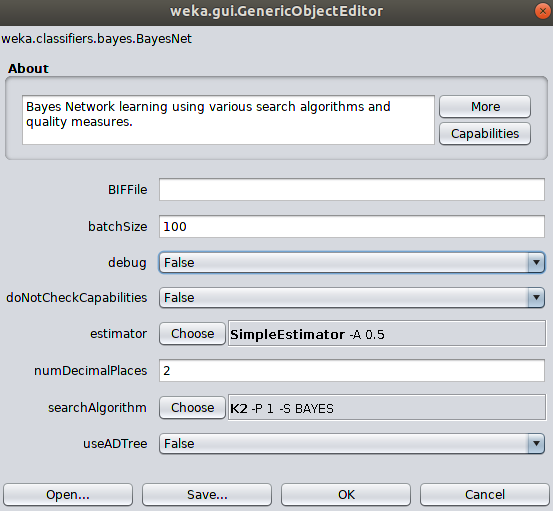
\includegraphics[scale=0.38]{Figures/3.png}
\caption{Algorisme de búsqueda K2}
\end{figure}

\newpage

\section{Model A}
\textit{\textbf{Xarxes bayesianes obtingudes amb K2 a partir d'un model inicial buit (sense arestes inicials) i amb un ordre entre les variables escollit a l'atzar i amb un valor determinat pel nombre màxim de pares per variable (paràmetre O en l'algoritme K2).}}\\
\begin{itemize}
\item Ajustem els paràmetres del K2 per satisfer les següents condicions:
	\begin{itemize}
	\item \textbf{Model inicial sense arestes}: \textit{initAsNaiveBayes} $\rightarrow$ \textit{False}
	\item \textbf{Ordre aleatori de selecció de variables}: \textit{randomOrder} $\rightarrow$ \textit{True}
	\item \textbf{Màxim nombre de pares per variable}: \textit{maxNrOfParents} $\rightarrow$ \textit{N, on N $\epsilon$  $\mathbb{N} - \{0\}$ }
	\end{itemize}
	\begin{figure}[hbtp]
	\centering
	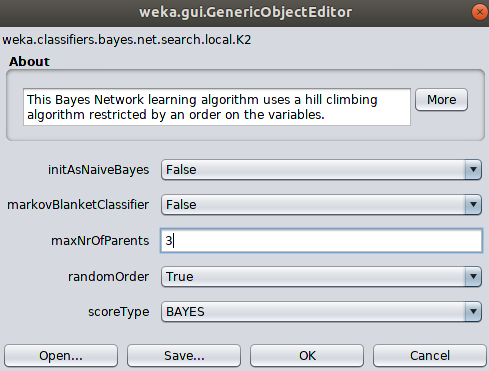
\includegraphics[scale=0.4]{Figures/5.png}
	\caption{Paràmetres K2 model A}
	\end{figure}
\item Visualitzem el graf generat en l'execució:
	\begin{figure}[hbtp]
	\centering
	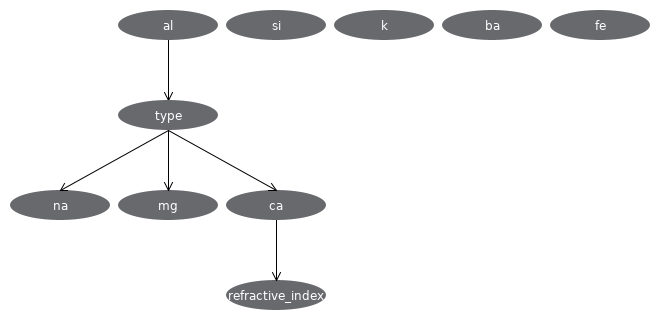
\includegraphics[scale=0.4]{Figures/r1.png}
	\caption{Graf aleatori generat amb els paràmetres del model A amb node arrel \textbf{si}}
	\end{figure}
\end{itemize}

\newpage

\section{Model B}
\textbf{\textit{Xarxa bayesiana naive (model únic), sent la variable de classe de vidre la variable independent (i pare de totes les altres). Per tant, el valor d'U en aquest cas haurà de ser 0.}}\\
\begin{itemize}
\item Ajustem els paràmetres del K2 per satisfer les següents condicions:
	\begin{itemize}
	\item \textbf{Type variable independent i pare de totes les altres}: \textit{initAsNaiveBayes} $\rightarrow$ \textit{True} i \textit{(Nom)} $\rightarrow$ \textit{Type}
	\item \textbf{Màxim nombre de pares per variable}:  
 \textit{maxNrOfParents} $\rightarrow$ \textit{0}
	\end{itemize}
	\begin{figure}[hbtp]
	\centering
	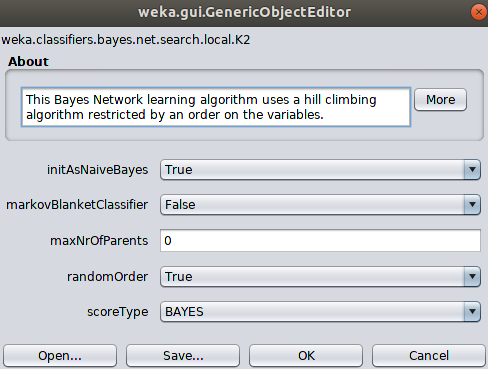
\includegraphics[scale=0.4]{Figures/6.png}
	\caption{Paràmetres K2 model B}
	\end{figure}

\item Visualitzem el graf generat en l'execució:
	\begin{figure}[hbtp]
	\centering
	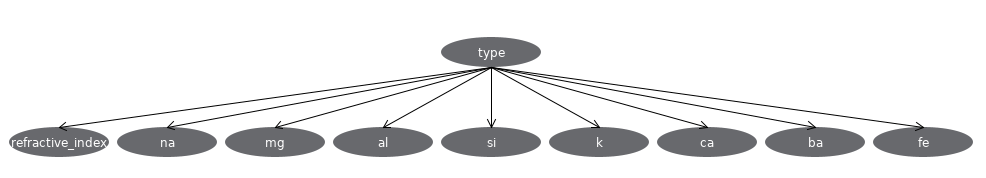
\includegraphics[scale=0.4]{Figures/r2.png}
	\caption{Graf aleatori generat amb els paràmetres del model B amb node arrel \textbf{type}}
	\end{figure}
\end{itemize}

\newpage

\section{Model C}
\textbf{\textit{Xarxes bayesianes obtingudes amb K2 a partir d'un model inicial que sigui la xarxa bayesiana naive del punt 2, però podent afegir arestes addicionals (i per tant U haurà de ser més gran que 0)}}
\begin{itemize}
\item Ajustem els paràmetres del K2 per satisfer les següents condicions:
	\begin{itemize}
	\item \textbf{Type variable independent i pare de totes les altres}: \textit{initAsNaiveBayes} $\rightarrow$ \textit{True} i \textit{(Nom)} $\rightarrow$ \textit{Type}
	\item \textbf{Màxim nombre de pares per variable}:  
 \textit{maxNrOfParents} $\rightarrow$ \textit{N, on N $\epsilon$  $\mathbb{N}$ }\\
	\end{itemize}
	\begin{figure}[hbtp]
	\centering
	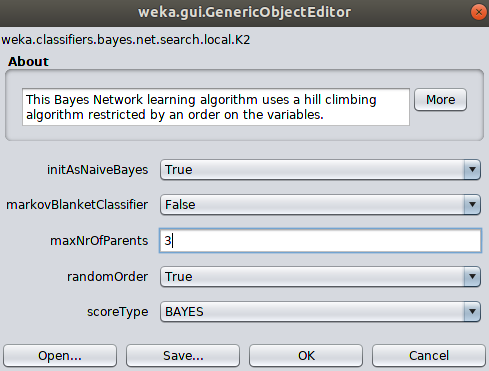
\includegraphics[scale=0.4]{Figures/4.png}
	\caption{Paràmetres K2 model C}
	\end{figure}
\item Visualitzem el graf generat en l'execució:\\
	\begin{figure}[hbtp]
	\centering
	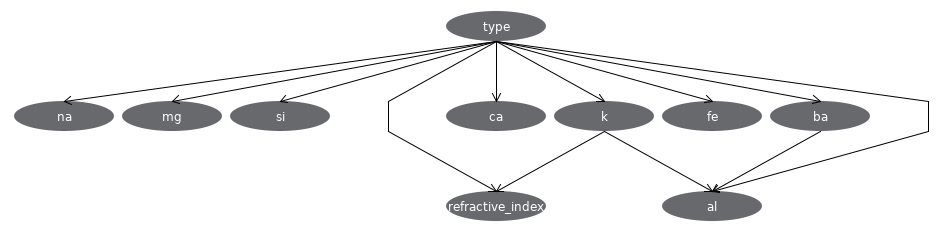
\includegraphics[scale=0.4]{Figures/r3.png}
	\caption{Graf aleatori generat amb els paràmetres del model C amb node arrel \textbf{type}}
	\end{figure}
\end{itemize}

\newpage

\part{10-fold Cross Validation}
\section{Generació train-folds}
Per tal de separar el training set i el test set hem utilitzat una proporció (10\% en aquest cas) per separar-los de forma aleatoria 10 vegades. D'aquesta forma simulem el \textit{folding} de 10 però cada cop la part del test podria incloure mostres de testos anteriors. L'script utilitzat es troba en la llibreta del codi font amb l'implementació degudament comentada.

\section{Evaluació test-folds}
\newpage

\part{Selecció del millor model}
\section{Model A}
\vspace*{0.5in}

\begin{table}[htbp]
\center
\begin{tabular}{|c||c|c|c|c|c|}
\hline
 & Fold 0 & Fold 1 & Fold 2 & Fold 3 & Fold 4 \\
\hline \hline
\textbf{Error \%}
 & 61.904 & 52.381 & 18.134 & 47.619 & 64.248\\
\hline
\textbf{LogScoreBayes} 
 & -3552.58 & -3654.07 & -3578.69 & -3594.25 & -486.30  \\
\hline
\end{tabular}
\caption{Errors de cada Fold pel model A - Part 1}
\end{table}

\vspace*{0.5in}

\begin{table}[htbp]
\center
\begin{tabular}{|c||c|c|c|c|c|}
\hline
 & Fold 5 & Fold 6 & Fold 7 & Fold 8 & Fold 9 \\
\hline \hline
\textbf{Error \%}
 & 38.095 & 57.142 & 47.619 & 57.142 & 52.381\\
\hline
\textbf{LogScoreBayes} 
 & -3614.40 & -3626.01 & -3664.74 & -3557.56 & -3637.68 \\
\hline
\end{tabular}
\caption{Errors de cada Fold pel model A - Part 2}
\end{table}

\vspace*{0.5in}

\begin{figure}[hbtp]
\centering
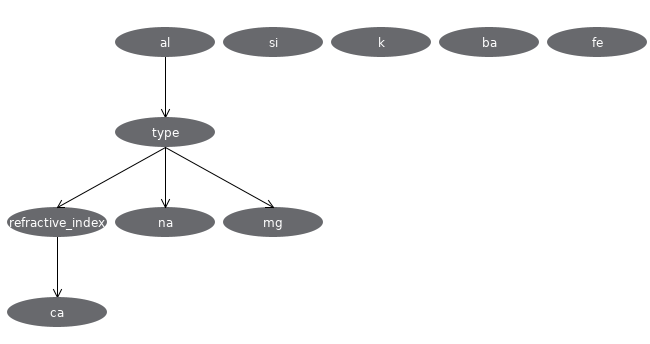
\includegraphics[scale=0.6]{Figures/r4.png}
\caption{Graf de la millor xarxa bayesiana obtinguda pel model A}
\end{figure}

\newpage

\section{Model C}
\vspace*{0.5in}

\begin{table}[htbp]
\center
\begin{tabular}{|c||c|c|c|c|c|}
\hline
 & Fold 0 & Fold 1 & Fold 2 & Fold 3 & Fold 4 \\
\hline \hline
\textbf{Error \%}
 & 90.476 & 61.904 & 38.079 & 57.142 & 90.476\\
\hline
\textbf{LogScoreBayes} 
 & -3738.98 & -3705.42 & -3717.93 & -3728.72 & -3698.30  \\
\hline
\end{tabular}
\caption{Errors de cada Fold pel model C - Part 1}
\end{table}

\vspace*{0.5in}

\begin{table}[htbp]
\center
\begin{tabular}{|c||c|c|c|c|c|}
\hline
 & Fold 5 & Fold 6 & Fold 7 & Fold 8 & Fold 9 \\
\hline \hline
\textbf{Error \%}
 & 71.428 & 61.904 & 76.190 & 61.904 & 80.952\\
\hline
\textbf{LogScoreBayes} 
 & -3735.10 & -3711.46 & -3707.39 & -3722.13 & -3732.31 \\
\hline
\end{tabular}
\caption{Errors de cada Fold pel model C - Part 2}
\end{table}

\vspace*{0.5in}

\begin{figure}[hbtp]
\centering
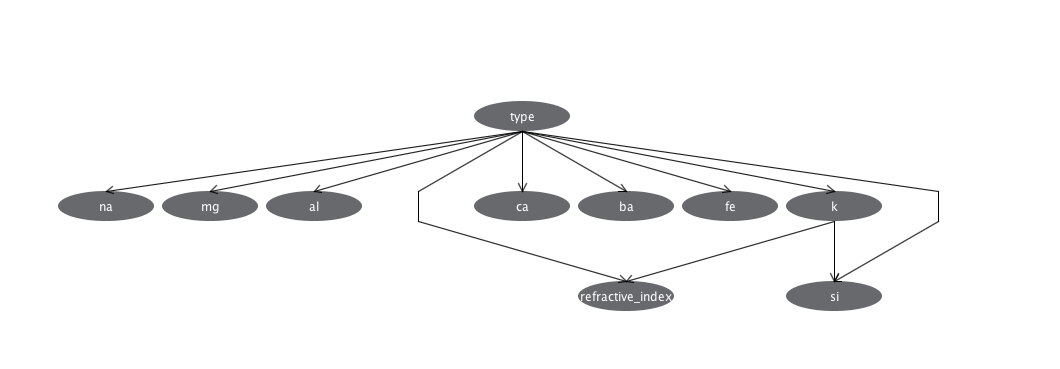
\includegraphics[scale=0.5]{Figures/r5.png}
\caption{Graf de la millor xarxa bayesiana obtinguda pel model C}
\end{figure}
\end{document}

